\documentclass[
	a4paper, 
	12pt, 
	brazilian
]{article}

\usepackage{config}

\begin{document}
	\section{Propriedades físicas da água I}
	
	\begin{itemize}
		\item\textbf{Massa específica}
			\begin{equation}
				\rho=f(\textrm{temperatura})
			\end{equation}
			\begin{equation}
				[\,\rho\,]=\left[\,\dfrac{m}{v}\,\right]=\SI{}{\dfrac{\kilogram}{\meter^{3}}}
			\end{equation}
			$\SI{4}{\SIUnitSymbolCelsius}\rightarrow\rho=\SI{1000}{\dfrac{\kilogram}{\meter^{3}}}$
			
			A \textbf{massa específica} da água é uma função de sua \textbf{temperatura}. Para outros fluidos as tabelas devem ser consultadas.	
			
			\textbf{Equação de Tanaka (2001):}
			Equação utilizada para determinar a densidade da água para variações de temperatura entre \SI{0}{\SIUnitSymbolCelsius} e \SI{40}{\SIUnitSymbolCelsius}.
			
			\begin{equation}
			\rho=999.974950\cdot\left(1-\dfrac{(T-3.983035)^{2}\cdot(T+301.797)}{522528.9\cdot (T+69.34881)}\right)
			\end{equation}	
		\item\textbf{Peso específico}
			\begin{equation}
				\gamma=\dfrac{W}{v}=\dfrac{m\cdot g}{v},\;\textrm{sendo}\;g=\SI{9.81}{\meter/\second^{2}}
			\end{equation}
			\begin{equation}
				[\,\gamma\,]=\SI{}{\dfrac{\newton}{\meter^{3}}}
			\end{equation}	
			A água a \SI{4}{\SIUnitSymbolCelsius} possui $\gamma=\SI{9810}{\newton/\meter^{3}}=\SI{1000}{kgf/\meter^{3}}$
			
			$\gamma$ pode ser reescrito como
			\begin{equation}
				\gamma=\rho\cdot g
			\end{equation}
		\item\textbf{Densidade (adimensional)}
		\begin{equation}
			d=\dfrac{\rho_{\textrm{substância}}}{\rho_{\textrm{padrão}}}
		\end{equation}
		A água a \SI{4}{\SIUnitSymbolCelsius} tem $d=1$, sendo utilizado como o padrão. Nessa temperatura $\rho_{\textrm{padrão}}=\SI{1000}{\kilogram/\meter^{3}}$.
		
		\item\textbf{Viscosidade:}
		\begin{itemize}
			\item[\textbf{(a)}] Coeficiente de viscosidade dinâmica
			
			Propriedade que confere resistência ao cisalhamento
			\begin{equation}
			\mu=f(\textrm{fluido, temperatura})
			\end{equation}
			\begin{equation}
			[\,\mu\,]=\SI{}{\pascal\cdot\second}
			\end{equation}
			Água a \SI{4}{\SIUnitSymbolCelsius} possui $\mu=\SI{1.566e-3}{\pascal\cdot\second}$
			
			\textbf{Equação de Lichachev (2003):}
			Calcula $\mu$ em função de $T$
			\begin{equation}
			\mu=32.025666\cdot 10^{-6}\cdot e^{\frac{482.134866}{T+119.886026}}
			\end{equation}
			
			\item[\textbf{(b)}] Coeficiente de viscosidade cinemática
				\begin{equation}
					\nu=f(\textrm{fluido, temperatura})
				\end{equation}
				\begin{equation}
					[\,\nu\,]=\left[\dfrac{\mu}{\rho}\right]=\SI{}{\dfrac{\meter^{2}}{\second}}
				\end{equation}
				\import{assets/tables}{viscosidade_cinematica_temperatura}
				\textbf{Unidades no Sistema C.G.S.}
				\begin{equation}
					[\,\mu\,]=\SI{}{\dfrac{dyn\cdot\second}{\centi\meter^{2}}}=\SI{}{P\,(poise)}
				\end{equation}
				\begin{equation}
					[\,\nu\,]=\SI{}{\dfrac{\centi\meter^{2}}{\second}}=\SI{}{St\,(stoke)}
				\end{equation}
		\end{itemize}
		\item\textbf{Compressibilidade}
		
		Proporciona redução do volume ocupado pelo fluido quando este é submetido a um incremento de pressão.
		
		\begin{figure}[H]
			\centering
			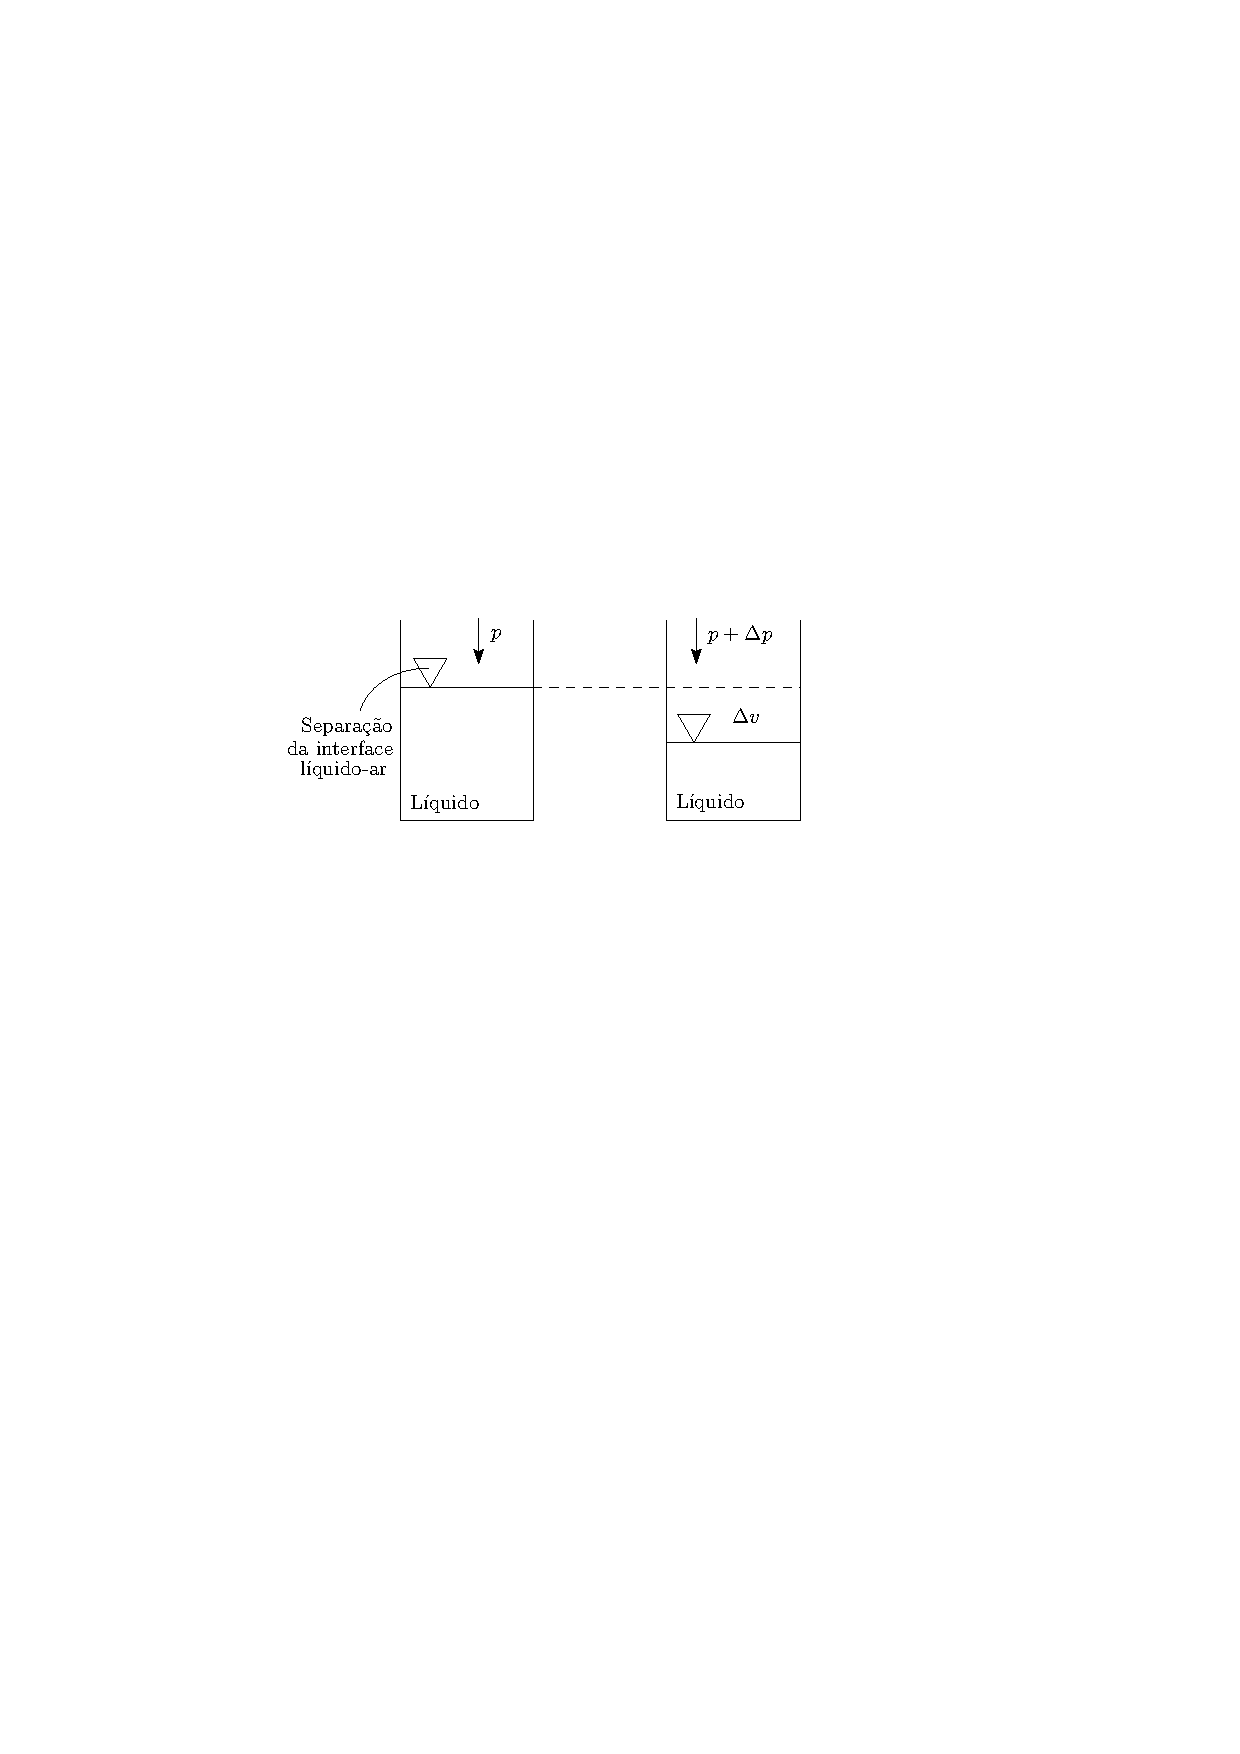
\includegraphics[width=0.7\linewidth]{assets/images/compressibilidade}
			\label{fig:compressibilidade}
		\end{figure}
		\begin{equation}
			\Delta v=-\alpha\cdot v_{1}\cdot\Delta p
		\end{equation}
		Água a \SI{20}{\SIUnitSymbolCelsius} tem $\alpha=\SI{4.75e-10}{\dfrac{\meter^{2}}{\newton}}$
		
		\item\textbf{Módulo de elasticidade}
		\begin{equation}
			E=\dfrac{1}{\alpha}
		\end{equation}
		Água a \SI{20}{\SIUnitSymbolCelsius} tem $E=\SI{21.07e8}{\pascal}$
		
		\textit{``Nas aplicações de hidráulica deve-se assumir que a água é um fluido incompressível.''}
	\end{itemize}

	\section{Propriedades físicas da água II}
	\begin{itemize}
		\item\textbf{Tensão superficial}
		
		Fenômeno em interface líquido-ar
		
		\textbf{Coesão:} Atração entre moléculas do próprio líquido.
		
		\textbf{Adesão:} Atração entre moléculas do líquido e do sólido com o qual há contato.
		
		\item\textbf{Ângulo de contato}
		\begin{enumerate}
			\item Água + superfície hidrofóbica
			\begin{figure}[H]
				\centering
				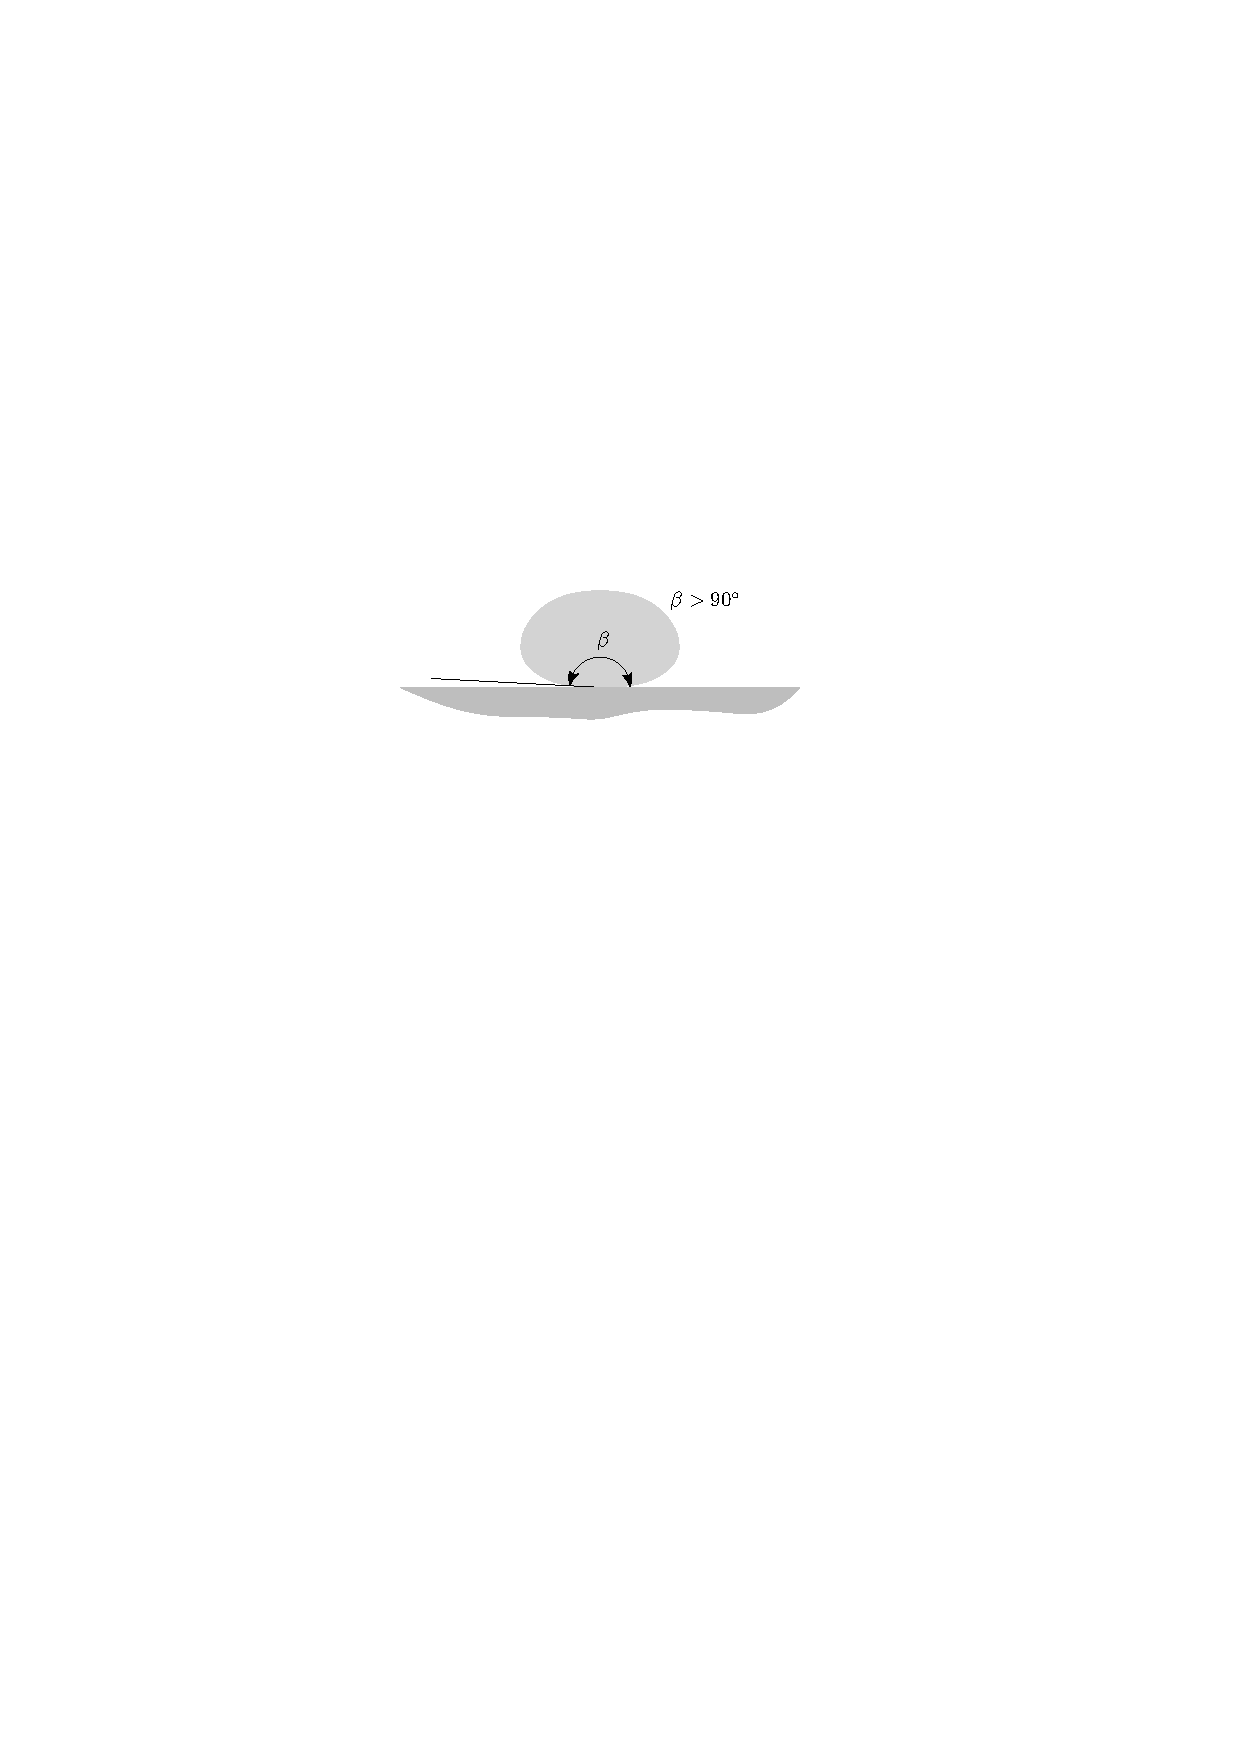
\includegraphics[width=0.5\linewidth]{assets/images/agua_superficie_hidrofobica}
				\label{fig:aguasuperficiehidrofobica}
			\end{figure}
			\item Água + superfície hidrofílica
			\begin{figure}[H]
				\centering
				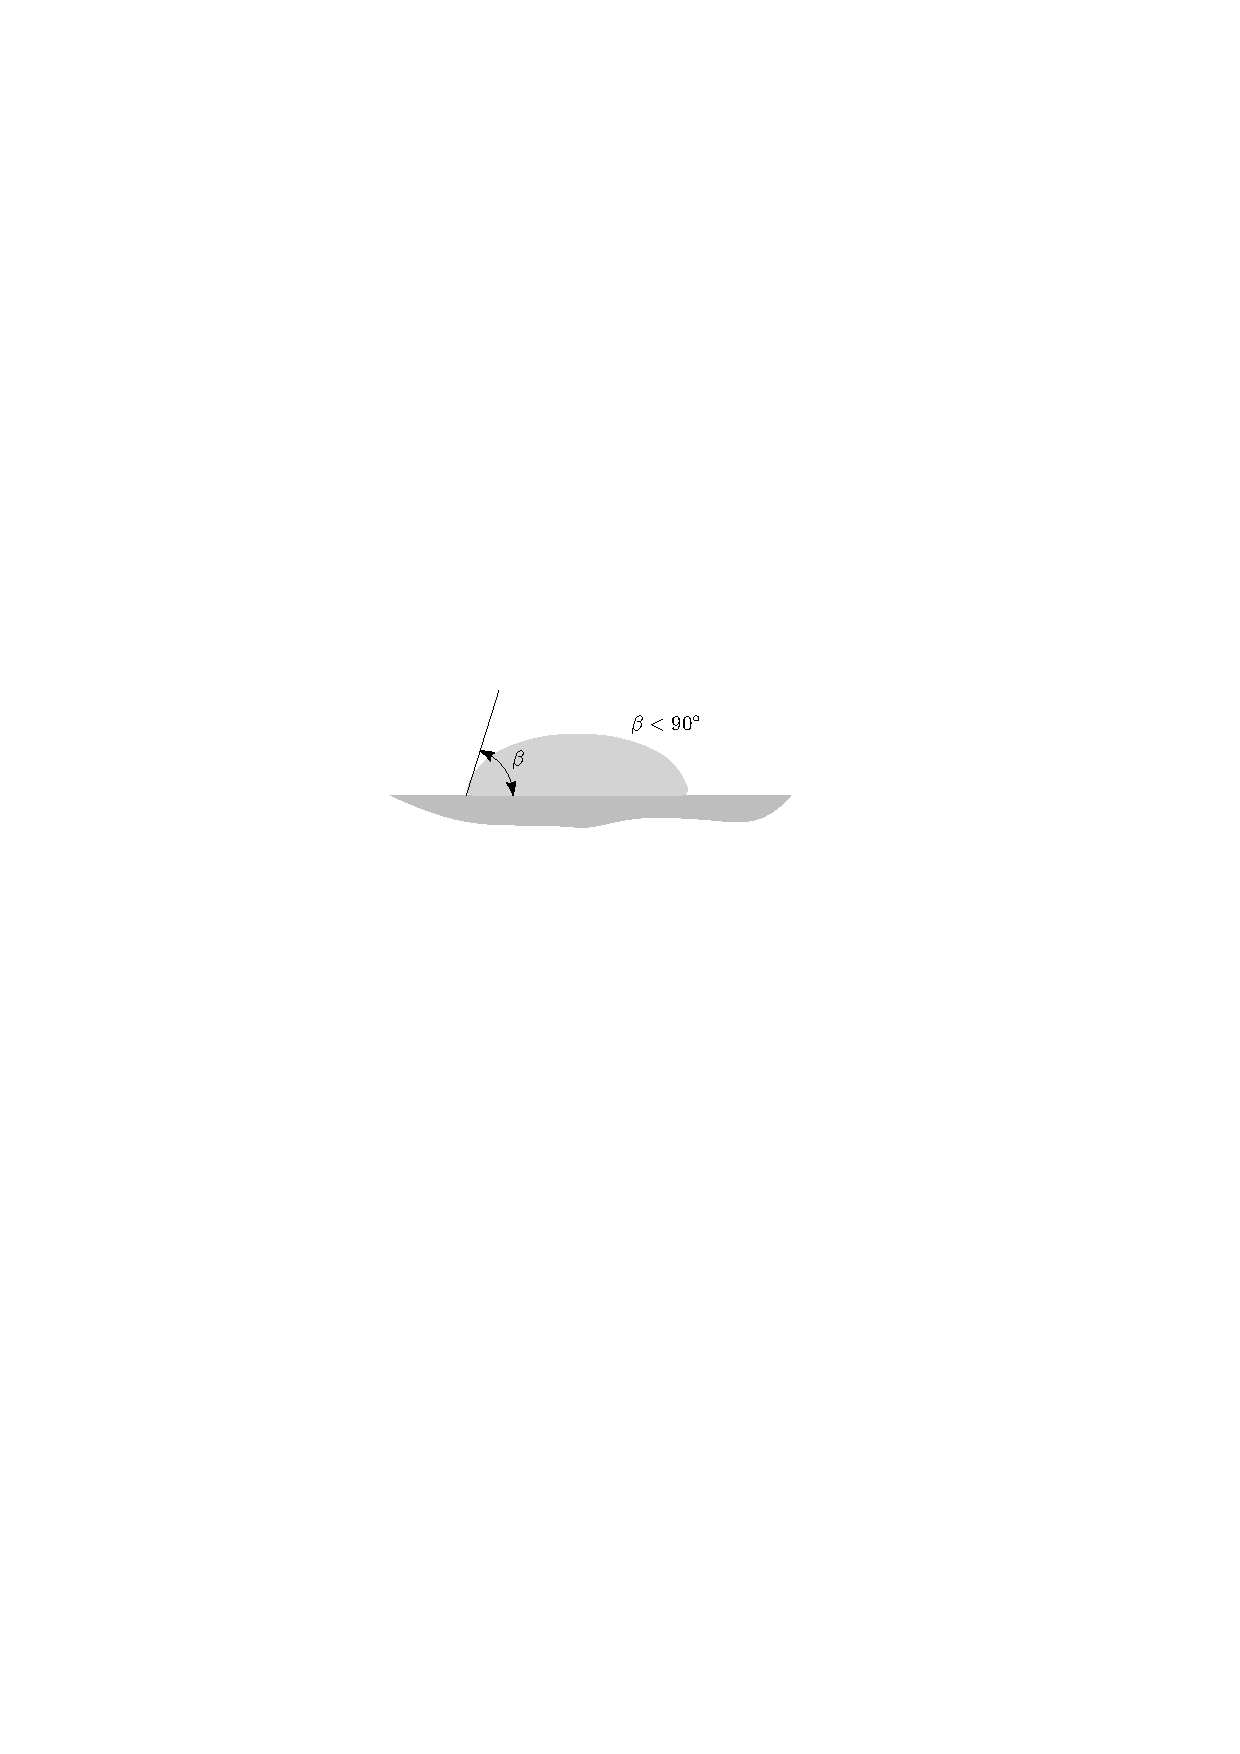
\includegraphics[width=0.5\linewidth]{assets/images/agua_superficie_hidrofilica}
				\label{fig:aguasuperficiehidrofilica}
			\end{figure}
			
			\begin{figure}[H]
				\centering
				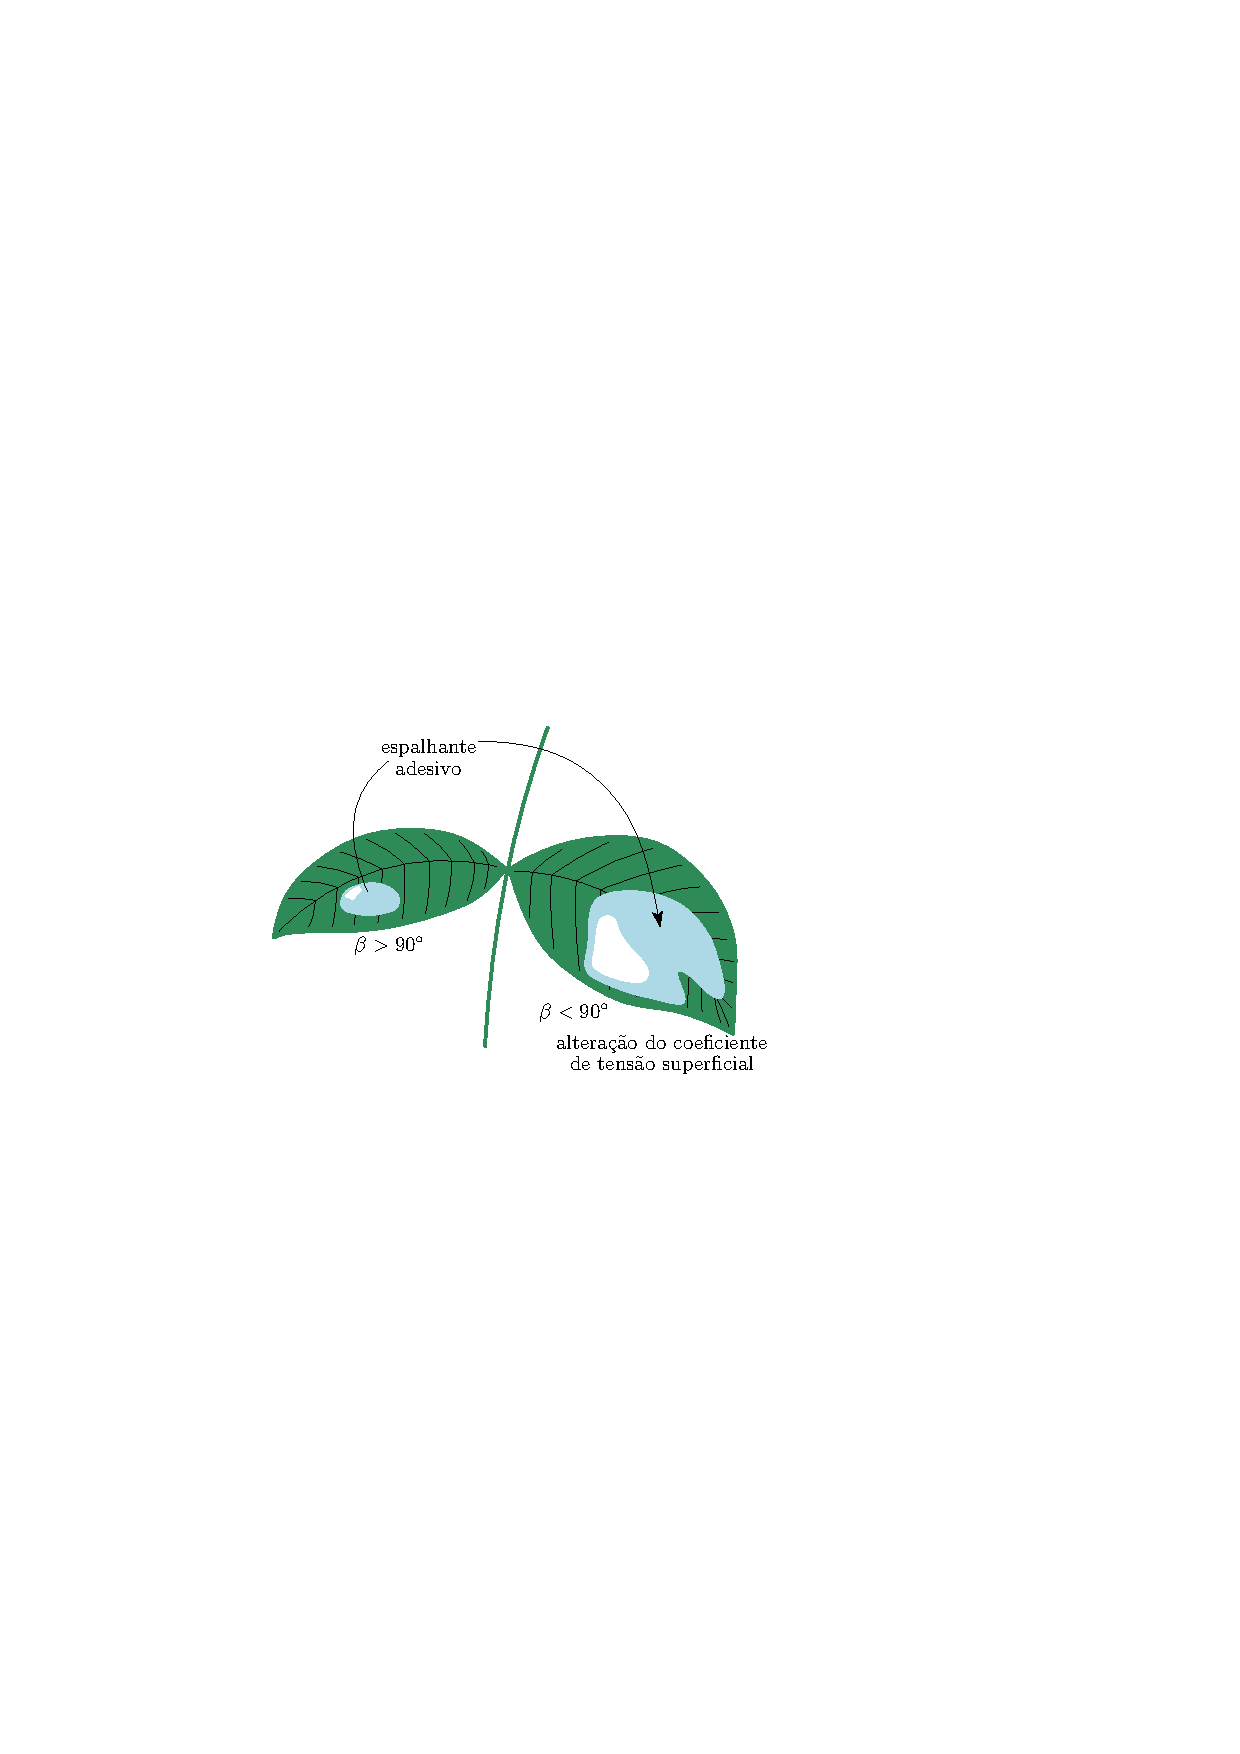
\includegraphics[width=0.7\linewidth]{assets/images/espalhante_adesivo}
				\label{fig:espalhanteadesivo}
			\end{figure}
		\end{enumerate}
		\item\textbf{Tensão superficial}
		\begin{equation}
			\sigma=f(\textrm{fluido, temperatura})
		\end{equation}
		Água a \SI{20}{\SIUnitSymbolCelsius} possui $\sigma=\SI{7.23e-2}{\dfrac{\newton}{\meter}}$
		
		\item\textbf{Capilaridade}
		
		Fenômenos de \textbf{ascensão} e \textbf{depressão} capilar
		
		\begin{figure}[H]
			\centering
			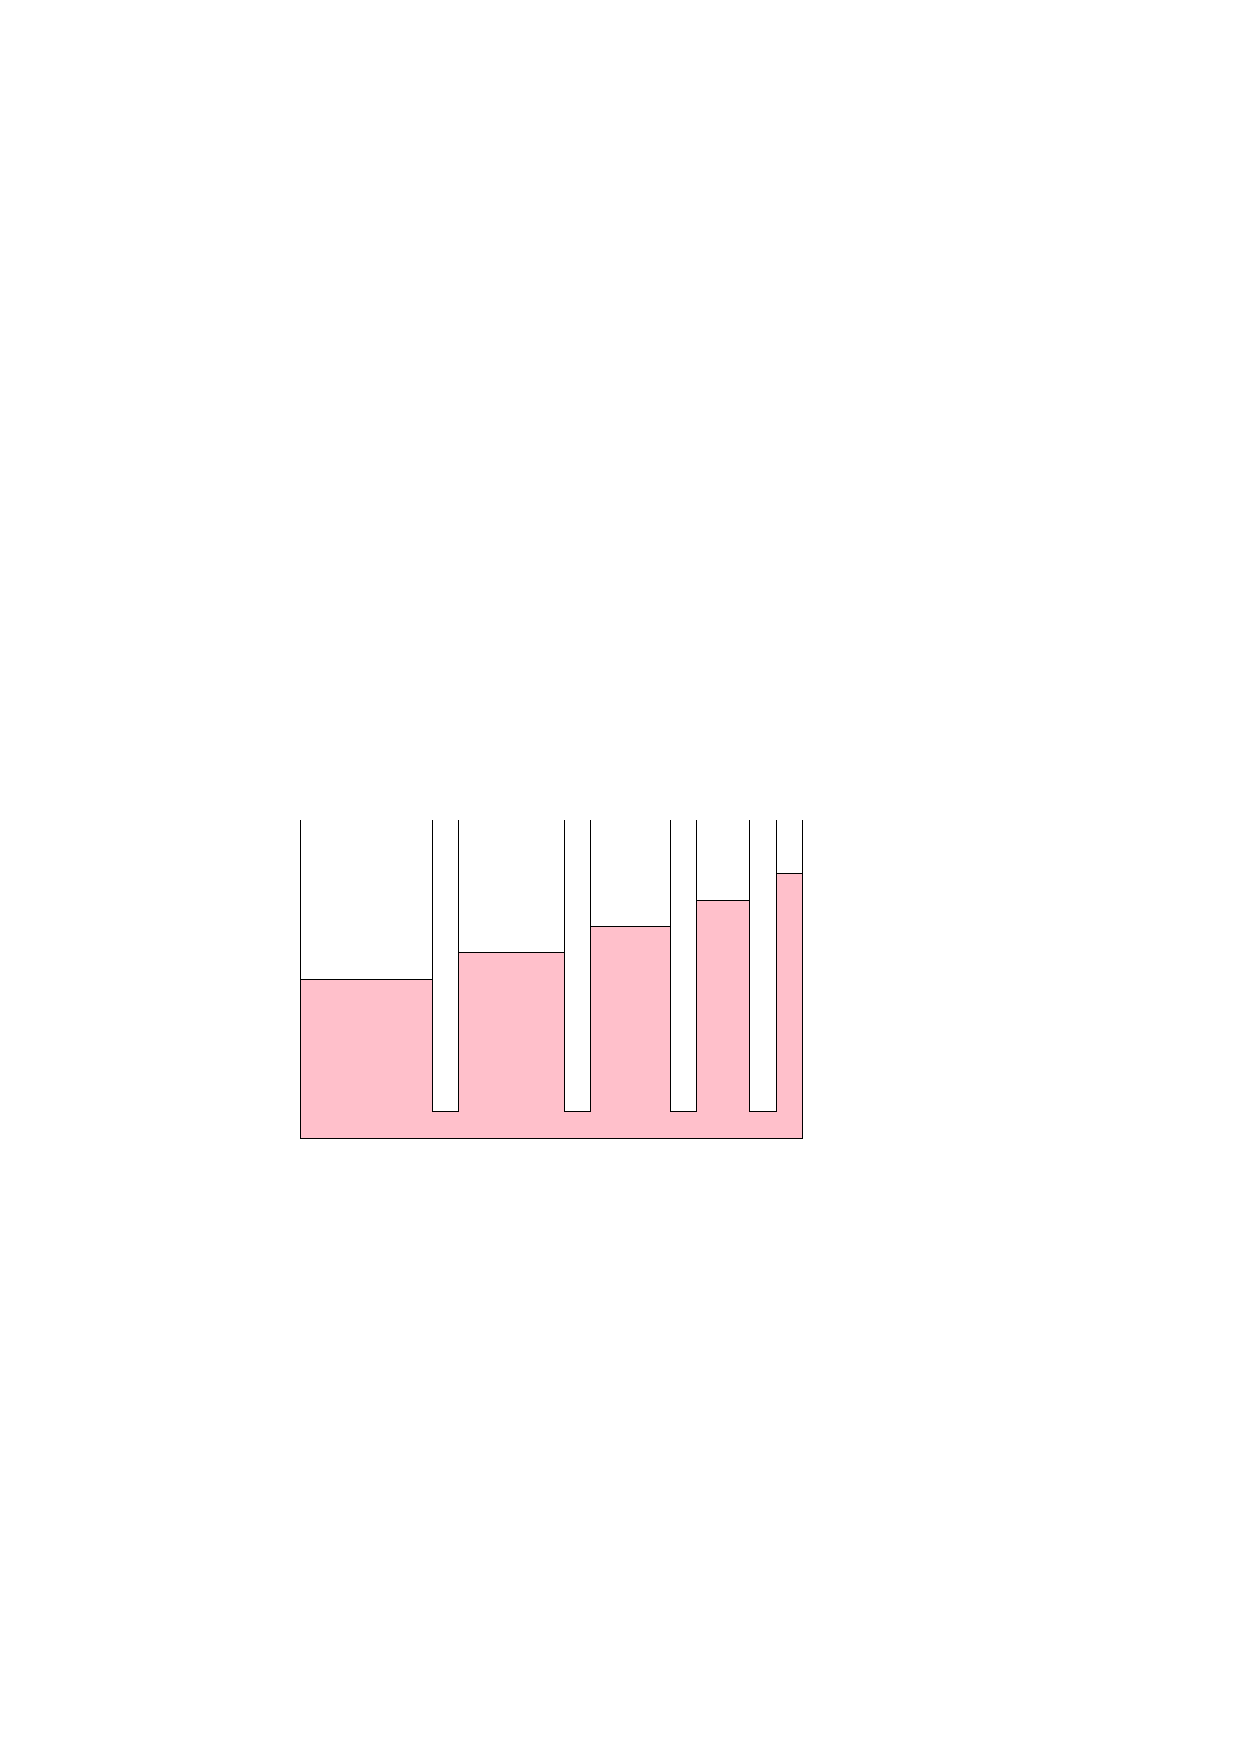
\includegraphics[width=0.5\linewidth]{assets/images/capilaridade}
			\label{fig:capilaridade}
		\end{figure}
		\begin{enumerate}
			\item Tubo capilar de vidro + água
			\begin{figure}[H]
				\centering
				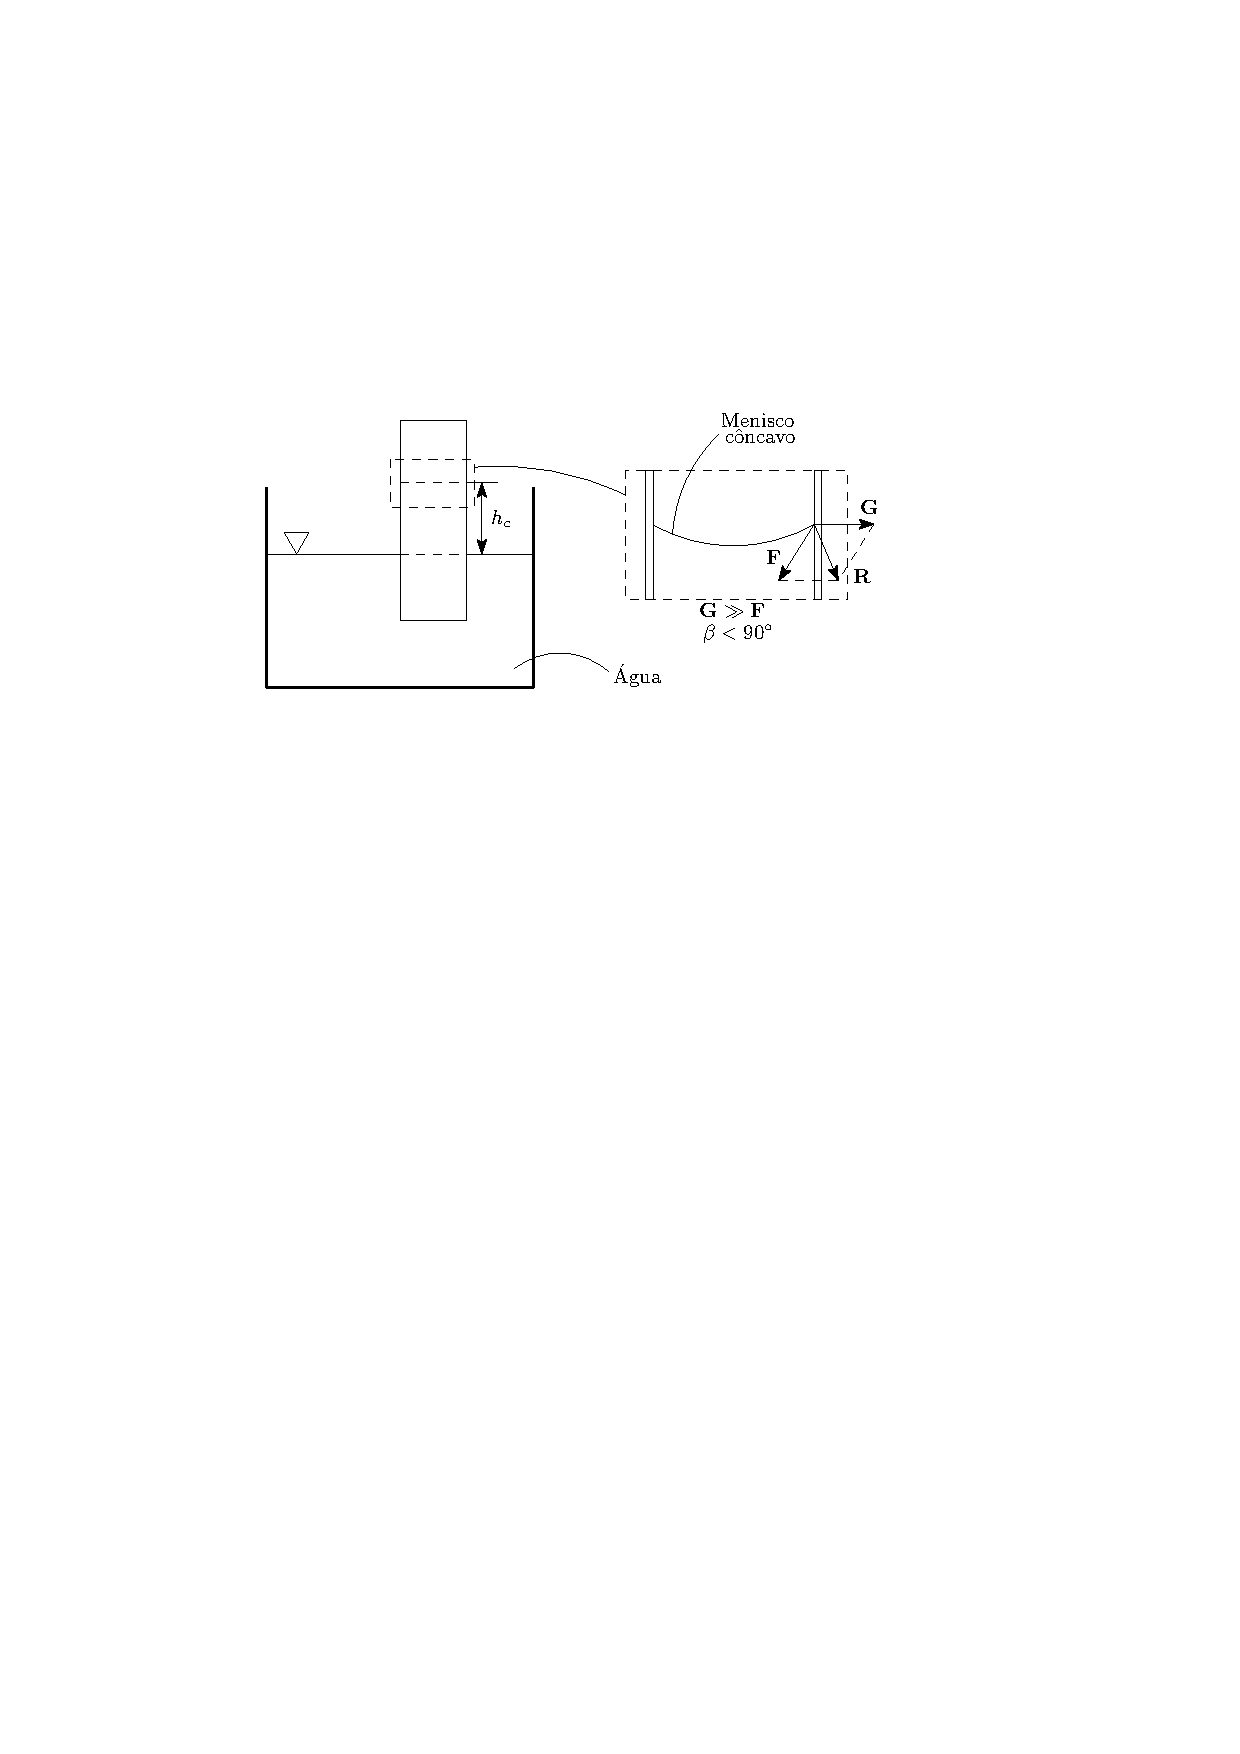
\includegraphics[width=0.8\linewidth]{assets/images/vidro_agua}
				\label{fig:vidroagua}
			\end{figure}
			\item Tubo capilar de vidro + mercúrio
			\begin{figure}[H]
				\centering
				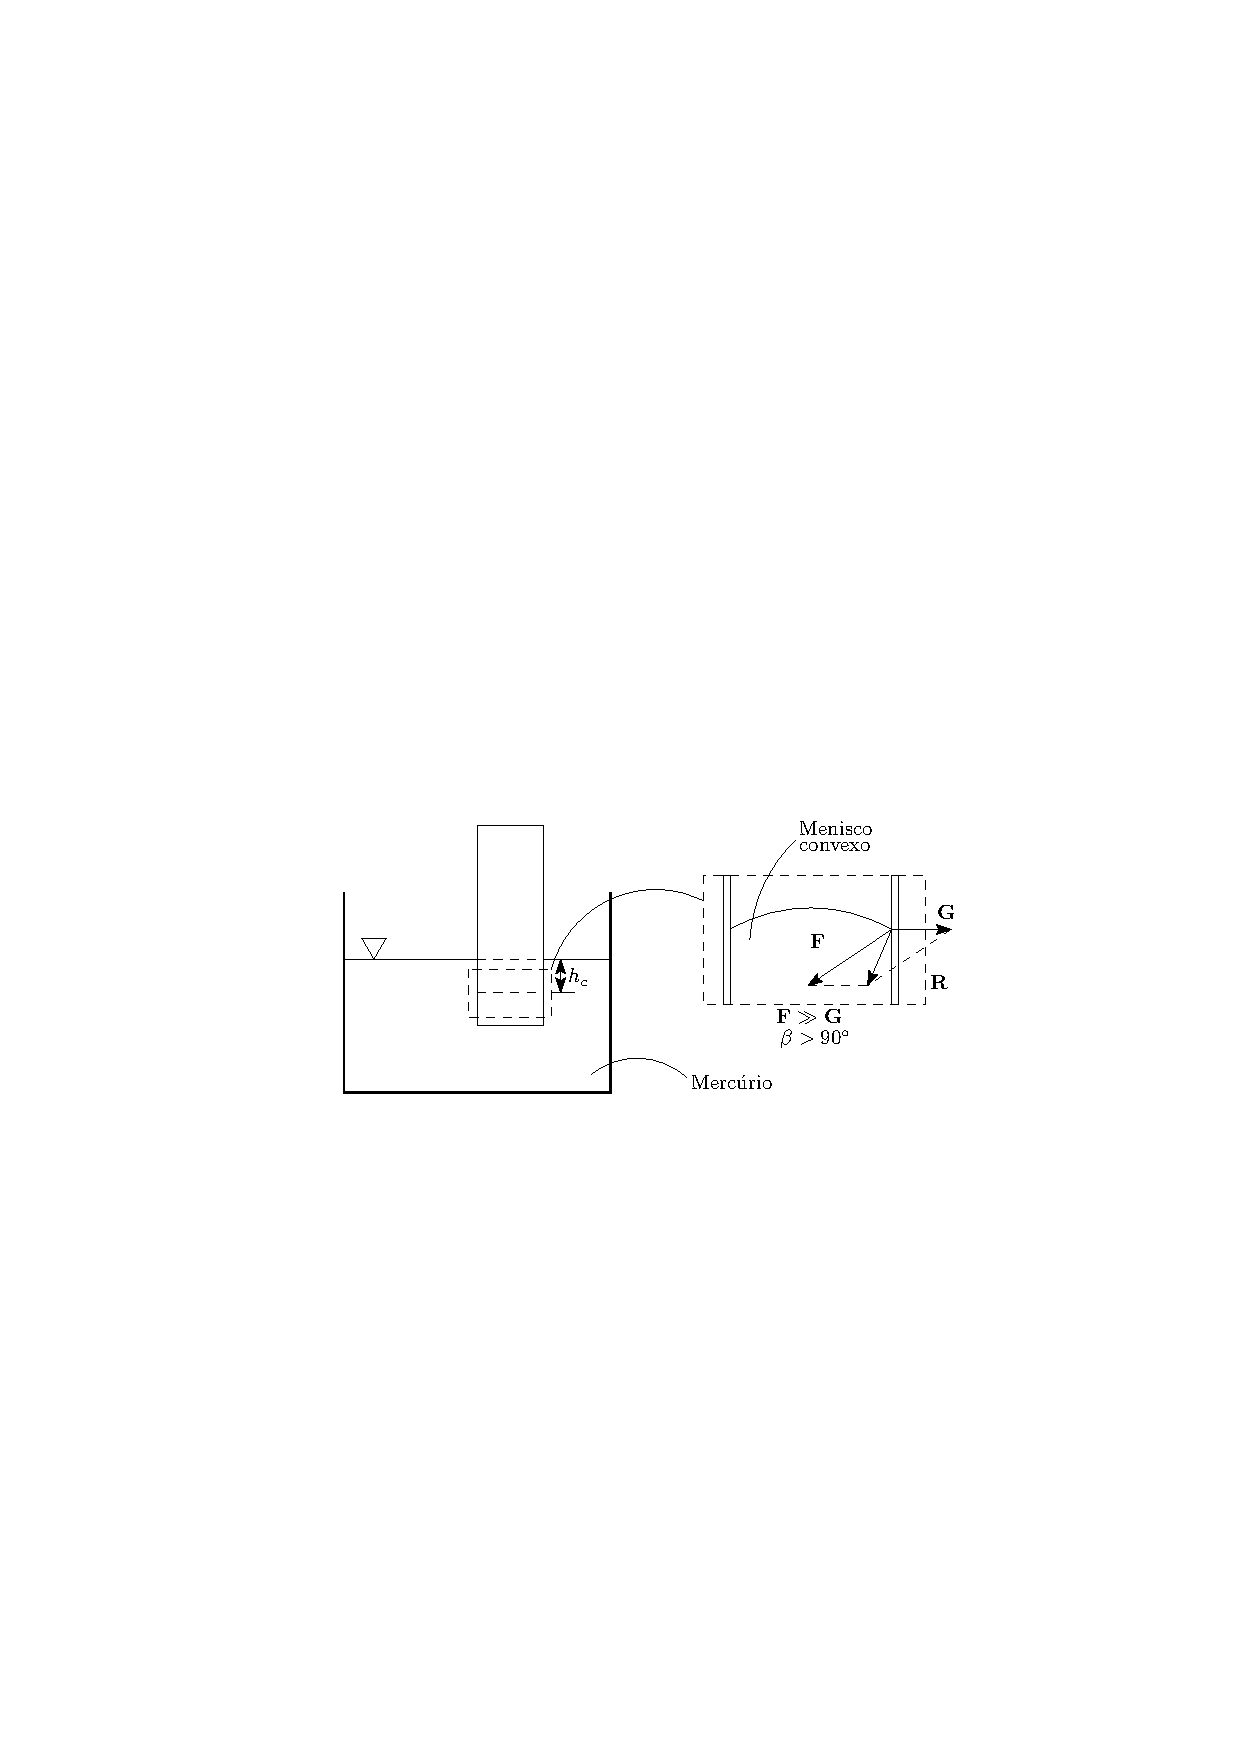
\includegraphics[width=0.8\linewidth]{assets/images/vidro_mercurio}
				\label{fig:vidromercurio}
			\end{figure}
			
		\end{enumerate}
		\textbf{Equação para cálculo da altura da ascensão/depressão capilar}
		\begin{equation}
			h_{c}=\dfrac{4\cdot\sigma\cdot\sin\beta}{\gamma\cdot d}
		\end{equation}
		$d$ é o diâmetro dos tubos capilares\\
		Solos arenosos: $\uparrow d\rightarrow\,\downarrow h_{c}$\\
		Solos argilos: $\downarrow d\rightarrow\,\uparrow h_{c}$
		
		\textbf{Comentários:}
		\begin{enumerate}
			\item Retenção e movimento de água no solo
			\item Fundamentos de hidrostática não se aplicam
			\item Diâmetro de piezõmetros para medição de pressão
		\end{enumerate}
		\item\textbf{Pressão de vapor:} É a pressão absoluta no qual ocorreria ebulição do líquido.
		\begin{equation}
			p_{v}=f(\textrm{fluido, temperatura, pressão absoluta})
		\end{equation}
		\import{assets/tables}{pressao_de_vapor}
		\import{assets/tables}{ponto_de_ebulicao}
	\end{itemize}
	\subsection{Resumo}
	\begin{enumerate}
		\item Massa específica
		\item Peso específico
		\item Densidade
		\item Viscosidade
		\item Compressibilidade
		\item Tensão superficial e capilaridade
		\item Pressão de vapor ($p_{\textrm{absoluta}}$)
	\end{enumerate}
\end{document}
